
% This is a LaTeX template for poster using University of Helsinki style
% This version uses pdflatex; if you have XeTeX available, consider using poster_xetex.tex for fancy font settings
%
% The official Graphical Instructions available from hy.logodomain.com (from university network only) defines colours, fonts etc. This Template does not perfectly match the official poster template of the university
%
% Jukka Suomela's collection of LaTeX tricks has been invaluable in building this template: http://cs.helsinki.fi/u/josuomel/latex/ 
%
% Template, sample content by Janne Korhonen

% Encoding of this file is iso-8859-1 latin 1

\documentclass[a4paper]{article} % This actually makes poster of size A4, scale up when printing. Used text font size is a bit small for A1 poster, preferably use \small in that case 

% Misc. packages
\usepackage[T1]{fontenc}
\usepackage{url}
\usepackage{amsfonts}
\usepackage[absolute]{textpos}
\usepackage{amssymb}
\usepackage{amsmath} 
\usepackage{amsthm}
\usepackage{framed}
% Graphics stuff
\usepackage[usenames,dvipsnames]{color}
\usepackage{tabularx}
\usepackage{amsmath}
\usepackage{amsthm}
\usepackage{amssymb}
\usepackage{multirow}
\usepackage{graphicx}
\usepackage{tikz}
\usetikzlibrary{shapes,fit,arrows,arrows.meta,calc,positioning,decorations}
\usepackage{booktabs}
\usepackage{algpseudocode}
\usepackage{algorithm}
\usepackage{framed}
\usepackage{complexity}
\usepackage{enumitem}
\usepackage{makecell}
\usepackage{multicol}

\newcommand{\allkbs}{\ensuremath{\mathbb{K}}} % set of all KBs
\newcommand{\kb}{\ensuremath{\mathcal{K}}} % KB
\newcommand{\realPos}{\ensuremath{\mathbb{R}^\infty_{\geq 0}}} % set of non-negative real numbers + inf 
\newcommand{\sig}{\ensuremath{\mathsf{At}}} % signature
\newcommand{\interp}{\ensuremath{\tau}} % interpretation
\newcommand{\allinterp}{\ensuremath{\Omega}} % set of interpretations
\newcommand{\modelSet}[1]{\ensuremath{\mathsf{Mod}(#1)}}    

% inconsistency measurement:
\newcommand{\inc}{\ensuremath{\mathcal{I}}} % inconsistency measure
\newcommand{\conten}{\ensuremath{\mathrm{c}}}
\newcommand{\forget}{\ensuremath{\mathrm{f}}}
\newcommand{\hitd}{\ensuremath{\mathrm{hit}}}
\newcommand{\sumd}{\ensuremath{\mathrm{sum}}}
\newcommand{\maxd}{\ensuremath{\mathrm{max}}}
\newcommand{\hs}{\ensuremath{\mathrm{hs}}}
\newcommand{\mcsc}{\ensuremath{\mathrm{mcsc}}}

% variable names:
\newcommand{\varAt}{\ensuremath{x}} % atom
\newcommand{\varFor}{\ensuremath{\phi}} % formula
\newcommand{\varSet}{\ensuremath{S}} % set

\newcommand{\TODO}[1]{\textbf{\textcolor{red}{TODO:} #1}}
\newcommand{\comment}[1]{\textcolor{dblue}{#1}}

\newcommand{\tseitinCls}[1]{\ensuremath{\mbox{Cls}(#1)}}
\newcommand{\tseitinVar}[1]{\ensuremath{\mbox{Var}(#1)}}
\newcommand{\tseitinEnc}[1]{\ensuremath{\langle #1 \rangle}}
\newcommand{\hardCls}{\ensuremath{F_{\mathrm{hard}}}}
\newcommand{\softCls}{\ensuremath{F_{\mathrm{soft}}}}

\newcommand{\copyFor}[1]{\ensuremath{{#1}^\prime}}
\newcommand{\copyOcc}[1]{\ensuremath{{#1}^o}}


\newcommand{\heading}[1]{{\sffamily\Large{\color{unigray}#1}}\vspace{4mm}}
\newcommand{\subheading}[1]{{\sffamily\normalsize{\color{sciorange}#1}}\vspace{2.5mm}}
\newcommand{\figwidth}{60mm}

\newcommand{\myframe}[5]{
\begin{textblock}{0}(#1,#2)
\tikzstyle{mybox}=[draw=unigray,fill=white,very thick,rectangle,rounded corners]
\tikzstyle{fancytitle}=[fill=white, text=unigray]
\begin{tikzpicture}
\small
\path[use as bounding box] (0,0) rectangle (0,0);
\draw [mybox] (-1.5mm,5mm) rectangle (#3*65mm-3.5mm,-5mm-#4mm);
\node[fancytitle, right=10pt] at (0mm,5mm) {\heading{#5}};
\end{tikzpicture}
\end{textblock}
}

\usetikzlibrary{arrows,shapes,positioning}

\setlist[itemize]{leftmargin=*}
\setlist[enumerate]{leftmargin=*}
\setlist{nosep,topsep=-\parskip}

% Fonts
%
% Palantino - Helvetica - Courier.
% I haven't really spent time to figure out how to best match the official university style with latex font packages, as I use XeTex myself...
\usepackage{mathpazo}
\linespread{1.10}
\usepackage[scaled]{helvet}
\usepackage{courier}

% Colours
\definecolor{sciorange}{RGB}{0,74,139}
\definecolor{unigray}{RGB}{140,140,140}
\definecolor{dblue}{HTML}{001C7F}
\definecolor{dorange}{HTML}{B1400D}
\definecolor{dgreen}{HTML}{12711C}
\definecolor{dred}{HTML}{8C0800}

% Textpos to manually position blocks of text on the page
\usepackage[absolute]{textpos}

% We define 1 mm grid for positioning the text blocks on the page
% The idea is to leave 10 mm marginals to all sides; the three text columns are 60 mm wide with 5 mm space between columns.
\setlength{\TPHorizModule}{1mm}
\setlength{\TPVertModule}{1mm}

% The origin is set to right below the main title; this means that main title blocks have negative y-coordinate. There is actually no good reason for this, I just happened to do this that way.
\textblockorigin{10mm}{45mm}

% parindent is set to zero, because it looks better in posters
% you could also add some space between paragraphs here, but I use manual vertical spaces in this sample
\setlength{\parindent}{0pt}


% Finally, the content
\begin{document}
\pagestyle{empty} % To get rid of page numbers and so


\begin{textblock}{95}(-4,-42)
%\includegraphics[width=20mm]{HY_flame.pdf}
%\hspace{-12pt}
%\includegraphics[width=50mm]{HY_text.pdf}

\includegraphics[width=60mm]{helsinki.png}
\end{textblock}

\begin{textblock}{95}(58,-38)

\includegraphics[width=38mm]{toulouse.jpg}
\end{textblock}

\begin{textblock}{95}(103,-37)

\includegraphics[width=40mm]{cyprus.png}
\end{textblock}

\begin{textblock}{95}(150,-37)

\includegraphics[width=40mm]{paris.png}
\end{textblock}

%\begin{textblock}{95}(132,-35)
%\includegraphics[width=58mm]{Uni_hagen_logo.png}
%\end{textblock}

% Main title
% If you need two lines for the title, you need to adjust the position of this block and textblockorigin
% Remember, two first words use faculty colour. If your title is long, you can use small letters.
\begin{textblock}{190}(0,-18)
\centering
{\sffamily\fontsize{14}{10}\selectfont{}{\textbf{A Versatile Framework for Formula-Based Enforcement\\and Synthesis in Abstract Argumentation}}}
\small \begin{center} Andreas Niskanen \quad Jean-Guy Mailly \quad Yannis Dimopoulos \quad Pavlos Moraitis \end{center} % If you have multiple authors, their names can be on the same line. Adjust font size as necessary
%\rule[2mm]{190mm}{0.3pt} % This is the line under the title, adjust the last parameter if it seems to be in the wrong place
\end{textblock}

% ------------------------------------------------------------------------------------------------------------------
% The "abstract" block. Does not actually exist in the university poster template, so you may consider not using this
\begin{textblock}{190}(0,-3)
\sffamily
\small

\begin{framed}
{\bf Motivation: } Argumentation frameworks (AFs) may need to be revised when new evidence shows that some conclusions are incorrect.\\
Existing approaches to \textbf{enforcement in abstract argumentation} mainly focus on \textbf{minimizing syntactic change} of the AF structure.\\
How to revise an AF to satisfy new \textbf{acceptance constraints} while minimizing unwanted changes to both the structure and conclusions?
\medskip

\textbf{Contributions:}

Unified framework for expressing semantic and syntactic constraints on AFs via weighted propositional formulas.\\
$\rightarrow$ \textbf{Generalization:} existing enforcement and synthesis notions captured as special cases while enabling new forms of enforcement.\\
$\rightarrow$  \textbf{Complexity analysis:} complexity results ranging from NP-completeness to $\Sigma_3^{\text{p}}$-completeness for major argumentation semantics.\\
$\rightarrow$ \textbf{Exact algorithm:} MaxSAT-based counterexample-guided abstraction refinement (CEGAR) approach for $\Sigma_2^{\text{p}}$-complete variants.\\ 
$\rightarrow$ \textbf{Empirical evaluation:} Scalability to moderately-sized AFs on a novel enforcement problem combining semantic and syntactic change.
\end{framed}
\end{textblock}

% ------------------------------------------------------------------------------------------------------------------
% Three-column stuff
%
% The vertical size of the columns depends on the content, so unfortunately you have to manually move contents around

% Graphics
% Use includegraphics with width same as the current block width
%\includegraphics[width=60mm]{zeros.png}

% Captions are in sans-serif font, with smaller typeface than the main text.
%\scriptsize\sffamily Complex zero points of polynomials with degree at most $8$ and coefficients in $\{ -1, 0, 1\}$.


% y-coordinates and heights of rows/frames
% \newcommand{\uy}{35}
% \newcommand{\uh}{66}
\newcommand{\uy}{45}
\newcommand{\uh}{67}
\newcommand{\ly}{111}
\newcommand{\lh}{116}
\newcommand{\fh}{190}
\newcommand{\ry}{232}

\small

% ----------------------- UPPER PART ----------------------------

\myframe{0}{55}{3}{\uh}{FORMULA-BASED ENFORCEMENT}


\begin{textblock}{78}(2,55)

\subheading{Instance}

$(\underbrace{\mathcal{A}}_{\text{arguments}}, \underbrace{\Phi^+, \Phi^-, \Phi^{\mathcal{R}}, w}_{\text{sets of weighted formulas}}, \underbrace{\sigma}_{\text{semantics}})$

\medskip

\begin{itemize}
    \item $\Phi^+$: What should happen \textbf{in at least one extension}?
    \item $\Phi^-$: What must not happen \textbf{in any extension}?
    \item $\Phi^{\mathcal{R}}$: Constraints on the \textbf{attack structure}.
    \item $w(\varphi) < \infty$: soft, $w(\varphi) = \infty$: hard constraint.
\end{itemize}

\medskip

\subheading{Task}

Find an AF $\mathcal{F} = (\mathcal{A}, \mathcal{R})$ which
\begin{itemize}
    \item satisfies all hard constraints, and
    \item minimizes the cost incurred by\\ not satisfying a soft constraint.
\end{itemize}
\end{textblock} 


\begin{textblock}{78}(85,55)

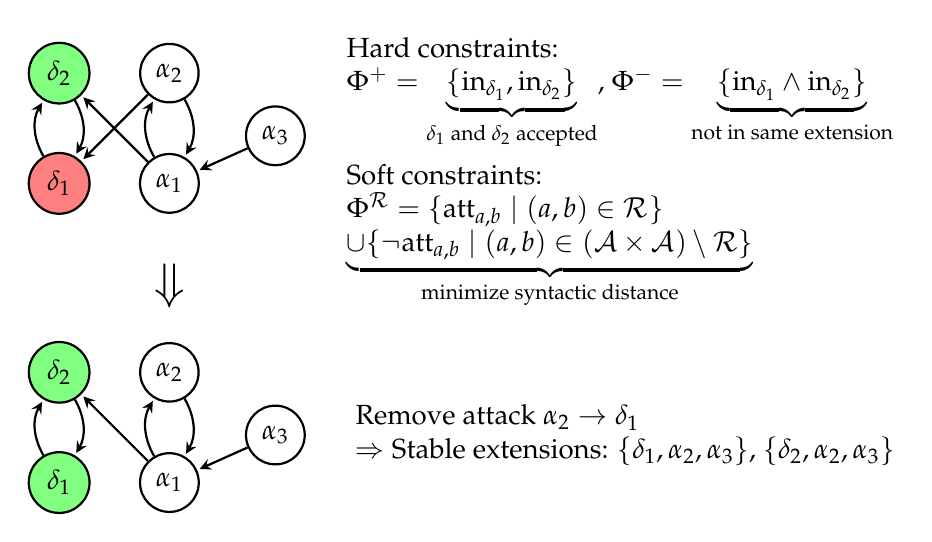
\begin{tikzpicture}[->,>=stealth,shorten >=1pt,auto,node distance=1.4cm, thick,main node/.style={circle,draw,font=\bfseries},uncertain/.style={rectangle,draw,dashed,font=\bfseries}]
    \node[main node,fill=red!50] (delta1) {$\delta_1$};
    \node[main node,fill=green!50] (delta2) [above of=delta1] {$\delta_2$};
    \node[main node] (alpha1) [right of=delta1] {$\alpha_1$};
    \node[main node] (alpha2) [right of=delta2] {$\alpha_2$};
    \node[main node] (alpha3) [below right=0.25cm and 0.8cm of alpha2] {$\alpha_3$};

    \path[->] (delta1) edge[bend left] (delta2)
        (delta2) edge[bend left] (delta1)
        (alpha2) edge (delta1)
        (alpha1) edge (delta2)
        (alpha3) edge (alpha1)
        (alpha1) edge[bend left] (alpha2)
        (alpha2) edge[bend left] (alpha1);

    \node[above right=-2.6cm and 0.5cm of alpha3,align=left] (phipm) {Hard constraints: \\ $\Phi^+ = \underbrace{\{\text{in}_{\delta_1}, \text{in}_{\delta_2}\}}_{\delta_1 \text{ and } \delta_2 \text{ accepted}}$, $\Phi^- = \underbrace{\{\text{in}_{\delta_1} \land \text{in}_{\delta_2}\}}_{\text{not in same extension}}$ \\ \\
    Soft constraints:\\
    $\Phi^{\mathcal{R}} = \{\text{att}_{a,b} \mid (a,b) \in \mathcal{R}\}$ \\ $\underbrace{\cup \{\neg \text{att}_{a,b} \mid (a,b) \in (\mathcal{A}\times\mathcal{A}) \setminus \mathcal{R}\}}_{\text{minimize syntactic distance}}$};

    \node[below=0.5cm of alpha1] {\LARGE$\Downarrow$};

    \node[main node,fill=green!50,below=3cm of delta1] (ddelta1) {$\delta_1$};
    \node[main node,fill=green!50] (ddelta2) [above of=ddelta1] {$\delta_2$};
    \node[main node] (aalpha1) [right of=ddelta1] {$\alpha_1$};
    \node[main node] (aalpha2) [right of=ddelta2] {$\alpha_2$};
    \node[main node] (aalpha3) [below right=0.25cm and 0.8cm of aalpha2] {$\alpha_3$};

    \path[->] (ddelta1) edge[bend left] (ddelta2)
        (ddelta2) edge[bend left] (ddelta1)
        (aalpha1) edge (ddelta2)
        (aalpha3) edge (aalpha1)
        (aalpha1) edge[bend left] (aalpha2)
        (aalpha2) edge[bend left] (aalpha1);

    \node[right=0.5cm of aalpha3,align=left] {Remove attack $\alpha_2 \to \delta_1$ \\ $\Rightarrow$ Stable extensions: $\{\delta_1,\alpha_2,\alpha_3\}$, $\{\delta_2,\alpha_2,\alpha_3\}$};

\end{tikzpicture} \\

\begin{tikzpicture}[->,>=stealth,shorten >=1pt,auto,node distance=1.4cm, thick,main node/.style={circle,draw,font=\bfseries},uncertain/.style={rectangle,draw,dashed,font=\bfseries}]

\end{tikzpicture}

\end{textblock}

\myframe{0}{126}{1.15}{61}{COMPLEXITY RESULTS}

\begin{textblock}{55}(2,127)

Formula-based enforcement generalizes\\
existing notions of extension enforcement\\
and status enforcement. \\
$\rightarrow$ Sustantial computational complexity.

\medskip

\begin{table}
    \centering
    \begin{tabular}{lc}
        \hline
        Semantics & Complexity \\
        \hline
        Grounded    & $\mathrm{NP}$-complete \\
        Admissible  & $\Sigma_2^{\text{p}}$-complete \\
        Complete    & $\Sigma_2^{\text{p}}$-complete \\
        Stable      & $\Sigma_2^{\text{p}}$-complete \\
        Preferred   & $\Sigma_3^{\text{p}}$-complete \\
        \hline
    \end{tabular}
\end{table}

\end{textblock}


\myframe{72.75}{126}{1.88}{100}{MAXSAT-BASED CEGAR ALGORITHM}

\begin{textblock}{115}(75,128)

\textbf{Focus:} $\Sigma_2^{\text{p}}$-complete variants (admissible, complete, and stable semantics).

\begin{enumerate}
    \item Solve \textbf{abstraction} as a MaxSAT instance:
    \begin{itemize}
        \item encode a witnessing $\sigma$-extension for each $\varphi \in \Phi^+$ as propositional clauses
        \item hard clauses: enforce each $\varphi \in \Phi^+ \cup \Phi^{\mathcal{R}}$ with $w(\varphi) = \infty$
        \item soft clauses: minimize cost over unsatisfied $\varphi \in \Phi^+ \cup \Phi^{\mathcal{R}}$ with $w(\varphi) < \infty$
    \end{itemize}
    \item Obtain optimal candidate AF and check for a \textbf{counterexample}:
    \begin{itemize}
        \item SAT solver call: is there an extension satisfying some $\varphi \in \Phi^-$?
    \end{itemize}
    \item If counterexample found: expand the abstraction by adding a \textbf{refinement clause}.
    \begin{itemize}
        \item Effectively reducing the search space requires \textbf{strong refinements}: account for changes in the structure which preserve the counterexample extension.
    \end{itemize}
\end{enumerate}

\end{textblock}

\begin{textblock}{70}(75,170)

\begin{center}
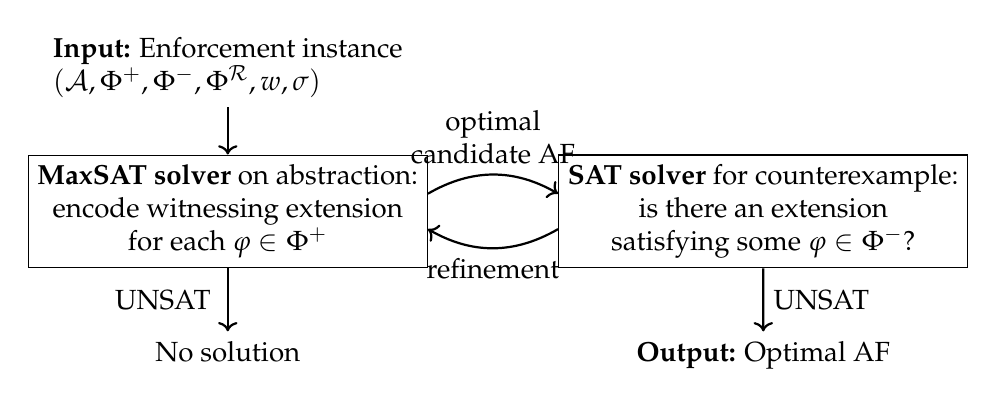
\begin{tikzpicture}[scale=0.8]
\node [align=center, draw] at (0,0) (RMP) {\textbf{MaxSAT solver} on abstraction: \\
encode witnessing extension \\ for each $\varphi \in \Phi^+$};
\node [align=center, draw] at (8.5,0) (PP) {\textbf{SAT solver} for counterexample: \\
is there an extension \\ satisfying some $\varphi \in \Phi^-$?};
\node [align=left, above=0.6 of RMP]  (I) { \textbf{Input:} Enforcement instance \\ $(\mathcal{A}, \Phi^+, \Phi^-, \Phi^{\mathcal{R}}, w, \sigma)$};
\draw [->, thick] (I.south) to (RMP.north);
\draw[->, thick] ([yshift=8pt] RMP.east) to[bend left] node[above,align=center] {optimal \\ candidate AF} ([yshift=8pt] PP.west);
\draw[->, thick] ([yshift=-8pt] PP.west) to[bend left] node[above,align=center] {} node[below,align=center] {refinement} ([yshift=-8pt] RMP.east);
\node [align=left, below=0.8 of PP] (O) {\textbf{Output:} Optimal AF};
\node [align=left, below=0.8 of RMP] (X) {No solution};
\draw [->, thick] (PP.south) to node[right,align=center] { UNSAT } (O.north);
\draw [->, thick] (RMP.south) to node[left,align=center] { UNSAT } (X.north);
\end{tikzpicture}
\end{center}

\end{textblock}

\myframe{0}{182}{1.15}{61}{EMPIRICAL EVALUATION}

%\begin{textblock}{70}(0,181)
\begin{textblock}{70}(0,178)

\begin{center}
Implementation available online in open source:

\smallskip

\scriptsize\url{https://bitbucket.org/andreasniskanen/phiaf}

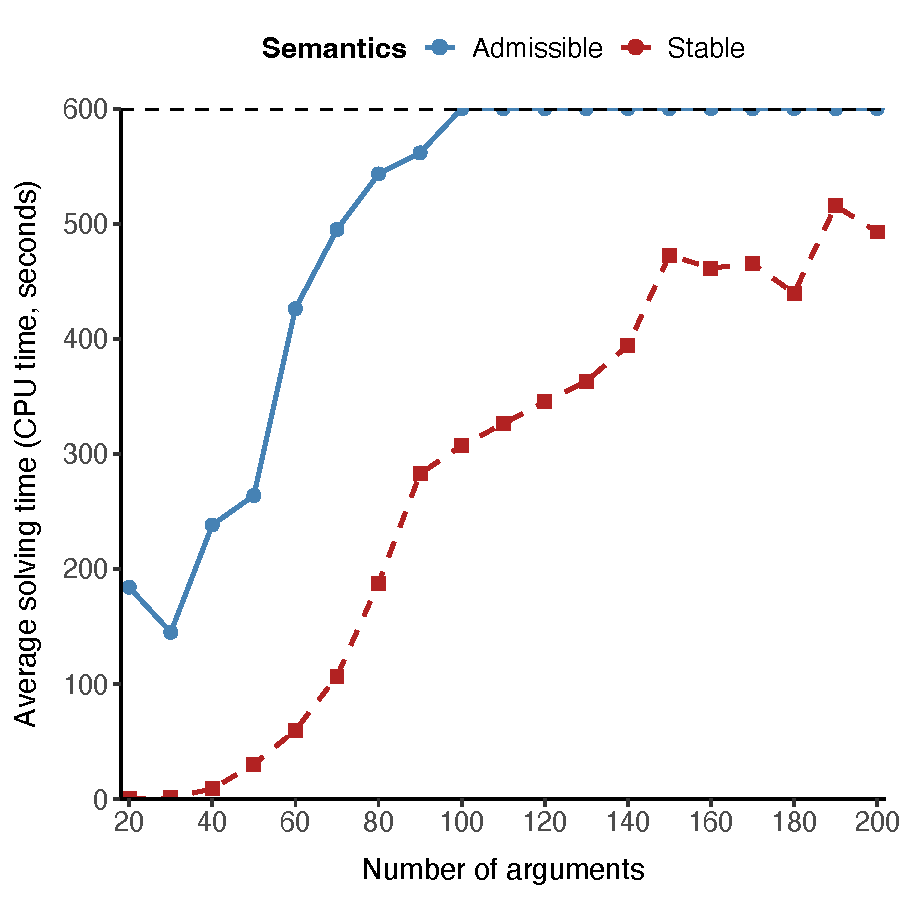
\includegraphics[width=0.82\textwidth]{solving_time_vs_arguments.pdf}

\end{center}

\end{textblock}

\myframe{72.75}{225}{1.88}{18}{REFERENCES}

\begin{textblock}{115}(74,225)

\scriptsize

Phan Minh Dung. On the acceptability of arguments and its fundamental role in nonmonotonic reasoning, logic programming and n-person games. \emph{Artif. Intell.}, 77(2):321–357, 1995

\smallskip

Ringo Baumann and Gerhard
Brewka. Expanding argumentation frameworks: Enforcing and monotonicity results. \emph{COMMA 2010},
75–86. IOS Press, 2010.

\smallskip

Andreas Niskanen, Johannes P.~Wallner, Matti Järvisalo. Optimal status enforcement in abstract argumentation. \emph{IJCAI 2016}, 1216-1222. AAAI Press, 2016.

\end{textblock}

\end{document}
